\documentclass[addpoints]{exam}
% \documentclass[addpoints,12pt]{exam}

\usepackage[slovene]{babel}
\usepackage{amsfonts}
\usepackage{amssymb}
\usepackage{amsmath}
\usepackage{float}
\usepackage{graphicx}
\usepackage{enumitem}
\usepackage{color}
\usepackage{eurosym}

\usepackage{pgfpages}
% \usepackage{tikz}
\usepackage{wrapfig}
\usepackage{pgfkeys}
\usepackage{pgfplots}
\usepackage{xcolor}
\usepackage{tkz-euclide}
\usepackage{xfp}




%Komentar naslednje vrstice glede na verzijo testa -- rešitve ali prostor za odgovore:
% \printanswers

% \linespread{2}


\pointsinrightmargin
\marginbonuspointname{}


\renewcommand{\solutiontitle}{\noindent\textbf{Rešitve in točkovanje:}\par\noindent}

\colorgrids
\definecolor{GridColor}{gray}{0.7}
\setlength{\gridsize}{7mm}

\extrawidth{5mm}
\setlength{\rightpointsmargin}{1.5cm}

\begin{document}

\runningfooter{}{}{}

\begin{center}
    \fbox{\fbox{\parbox{15cm}{\centering
    Popravljanje in pridobivanje ocen -- konferenca \\ 2. letnik -- test D \\ 15. junij 2026 \\ (Potence in koreni; Funkcija; Potenčna, korenska in kvadratna funkcija; Kompleksna števila)}}}
\end{center}

\vspace{0.1in}
\makebox[\textwidth]{Ime in priimek, oddelek:\enspace\hrulefill}


\begin{center}
    \hqword{Naloga}
    \hpword{Možne točke}
    \chbpword{Dodatne točke}
    \hsword{Dosežene točke}
    \htword{Skupaj}  
    % \combinedpointtable[h][questions]
    \gradetable[h][questions]

\end{center}

\vspace{0.1in}


\begin{questions}

    % 1. vprašanje

    \question[5]
    Izračunajte natančno vrednost izraza. 
    $$ \sqrt[4]{ 216^{\frac{2}{3}} + 0.125^{-2}} - \left(3+\sqrt{3}\right)\sqrt{12-6\sqrt{3}}$$ % - \dfrac{1+\sqrt{12}}{2+\sqrt{3}} $$

    \begin{solution}[7cm]
       
    \end{solution}


    % 2. vprašanje

    % \question[6]
    % Rešite enačbo. 
    % $$ \sqrt{3x-2} + 2 = 2\sqrt{x+2} $$

    % \begin{solution}[5.25cm]
       
    % \end{solution}

    \question
    Na sliki je graf funkcije $g$, ki smo ga dobili s transformacijo grafa funkcije $f(x)=\sqrt{x}$.
    
    \begin{figure}[H]
        \centering
        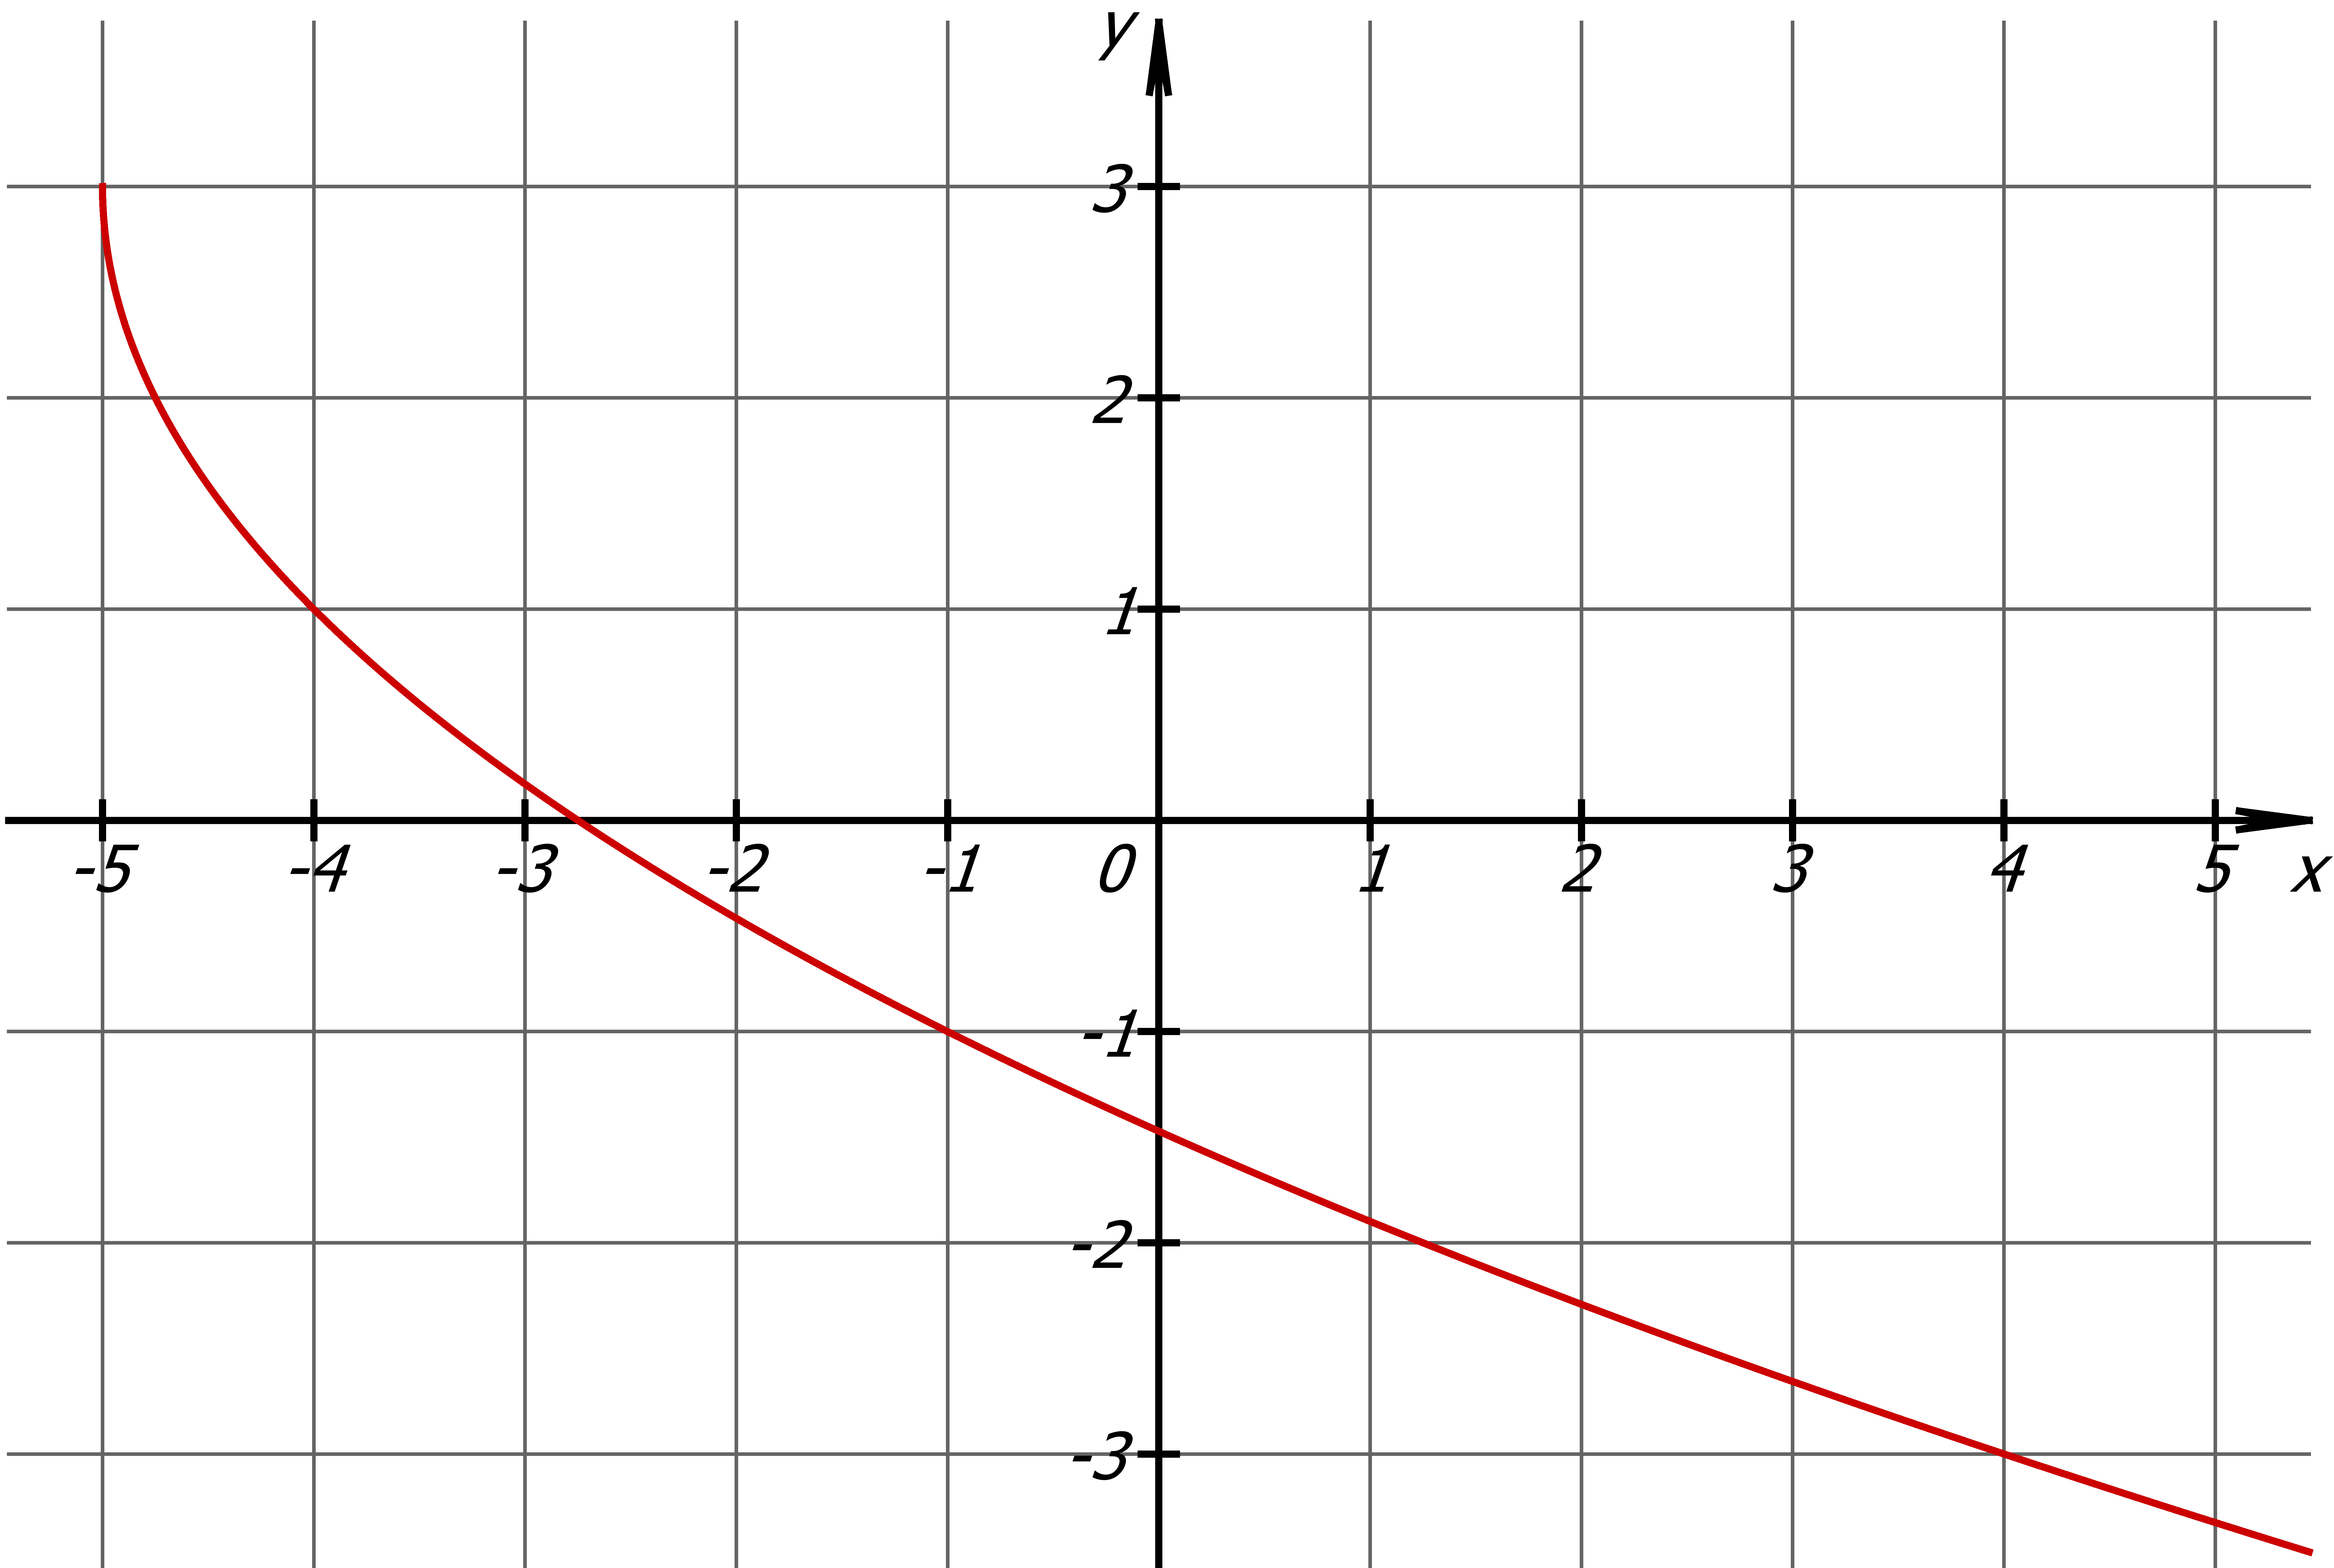
\includegraphics[scale=0.04]{test3_korenska.png}
    \end{figure}

    \begin{parts}
        \part[2] 
        Na zgornjo sliko dorišite graf funkcije $h(x)=\lvert g(x-1)\rvert$.
        
            \begin{solution}

            \end{solution}        

        % \part[4]
        % Zapišite predpis funkcije $g$, če njen graf poteka skozi točko $(11,-5)$.

        %     \begin{solution}[7cm]

        %     \end{solution}

    
        % \part[1]
        % Zapišite predpis funkcije $p(x)=-2 f(x-2)$.
        
        %     % \begin{solution}[5cm]

        %     % \end{solution}


    \end{parts}

\newpage
    % 3. vprašanje

    \question
    Dana je funkcija $f(x)=\left(x-1\right)^{-3}-1$.

    \begin{parts}
        \part[1]
        Zapišite definicijsko območje $D_f$ funkcije $f$. 

            \begin{solution}[1.5cm]

            \end{solution}
        
        % \part[4] 
        % Izračunajte ničle in začetno vrednost funkcije $f$.
    
        %     \begin{solution}[6cm]

        %     \end{solution}

        % \part[2] 
        % Ali je funkcija $f$ soda ali liha? Utemeljite.
    
        %     \begin{solution}[5cm]

        %     \end{solution}

        % \part[2] 
        % Zapišite enačbi vodoravne in navpične asimptote funkcije $f$.
    
        %     \begin{solution}[2.5cm]

        %     \end{solution}

        % \part[2] 
        % Določite presečišča grafa funkcije $f$ s premico $x=0$.
    
        %     \begin{solution}[4cm]

        %     \end{solution}


        \part[5] 
        Narišite graf funkcije $f$.
    
            \begin{solution}[12cm]

            \end{solution}
            
    \end{parts}


    

    % \newpage
    % 4. vprašanje
    \question[4]
    Dana je družina parabol $y=2x^2+(3-m)x+2$.
    Določite vrednost parametra $m$ tako, da bo imela parabola z abscisno osjo eno skupno točko.
    % \begin{parts}
        
    %     \part[6]
        % Določite vrednost parametra $m$ tako, da bo imela parabola z abscisno osjo eno skupno točko.
        % Določite tudi točko dotikališča.

            \begin{solution}[6cm]

            \end{solution}




\newpage
    % 1. vprašanje

    \question
    Dana je kvadratna funkcija $f(x)=\frac{1}{4}x^2-\frac{1}{4}x-\frac{15}{16}$.

    \begin{parts}
        
        % \part[4]
        % Zapišite predpis funkcije $f$ v ničelni obliki.

        %     \begin{solution}[8cm]

        %     \end{solution}

            
        \part[4]
        Zapišite predpis funkcije $f$ v temenski obliki.

            \begin{solution}[7cm]

            \end{solution}


        % \newpage
        % \part[1]
        % Določite začetno vrednost funkcije $f$.

        %     \begin{solution}[3cm]

        %     \end{solution}

        % \part[2]
        % Določite definicijsko območje in zalogo vrednosti funkcije $f$.

        %     \begin{solution}[3cm]

        %     \end{solution}

        % \part[2]
        % Določite enačbo simetrijske osi grafa funkcije $f$.

        %     \begin{solution}[2cm]

        %     \end{solution}


        % \part[5]
        % Narišite graf funkcije $f$.

        %     \begin{solution}[5cm]

        %     \end{solution}
        

        % \newpage
        
        \part[4]
        Graf funkcije $f$ togo premaknemo za vektor $\vec{v}=(-0.5,1)$ in tako dobimo graf funkcije $g$.
        Določite predpis funkcije $g$.

            \begin{solution}[5cm]

            \end{solution}


        % \part[3]
        % Določite predpis funkcije $h$, katere graf dobimo, če graf funkcije $f$ raztegnemo za faktor $3$ vzdolž ordinatne osi ter zrcalimo preko ordinatne osi.

        %     \begin{solution}[7cm]

        %     \end{solution}


    \end{parts}


    % \newpage
    % 2. vprašanje

    % \question[4]
    % Dana je družina parabol $y=2x^2+(3-m)x+2$.
    % Določite vrednost parametra $m$ tako, da bo imela parabola z abscisno osjo eno skupno točko.
    % % \begin{parts}
        
    % %     \part[6]
    %     % Določite vrednost parametra $m$ tako, da bo imela parabola z abscisno osjo eno skupno točko.
    %     % Določite tudi točko dotikališča.

    %         \begin{solution}[11cm]

    %         \end{solution}


        % \part[4]
        % Določite $m$ tako, da parabola z abscisno osjo ne bo imela skupnih točk.

        %     \begin{solution}[6cm]

        %     \end{solution}


        % \part[2]
        % Za katero vrednost parametra $m$ enačba predstavlja parabolo? 
        % Določite presečišče parabole z ordinatno osjo.

        %     \begin{solution}[2cm]

        %     \end{solution}


    % \end{parts}



    

% \newpage

    % 1. vprašanje
    % \question[5]
    %     Dani sta družina parabol $y=(2a+1)x^2-12x+9$ in parabola $y=-x^2+2x-3$.
    %     Kateremu pogoju mora ustrezati parameter $a$, da se paraboli dotikata?
    %     % Določite enačbo parabole.

    %         \begin{solution}[9cm]

    %         \end{solution}


    % 2. vprašanje
    % \question
    %     Miha vrže z okna svoje sobe v zrak kovanec. Funkcija $h$, s predpisom $h(t)=-5t^2+10t+15$, 
    %     opisuje višino kovanca v odvisnosti od časa. Čas je merjen v sekundah, višina pa v metrih.
        
    %     \begin{parts}
    %         \part[1] S katere višine je Miha vrgel kovanec?
    %         % \part[3] Po kolikšnem času pade kovanec na tla?
    %         % \part[2] Kolikšna je največja višina kovanca med letom?
    %     \end{parts}

    %         \begin{solution}[2cm]

    %         \end{solution}

    % 4. vprašanje
    \question[5]
        V kompleksni ravnini upodobite množico točk:                     
            $$\left\{z\in\mathbb{C}; \left|Re(z)\right|>2 \land \left|z\right|\leq 4 \right\}. $$ 
        
            \begin{solution}[6cm]

            \end{solution}

            \newpage
    % 3. vprašanje
    \question
        Dano je kompleksno število $$z= \dfrac{5+3i}{3-5i}-i^{39}-\left(2+i\sqrt{3}\right)\left(2-i\sqrt{3}\right). $$

        \begin{parts}
            
            \part[5]
            Poenostavite zapis kompleksnega števila $z$.

                \begin{solution}[16cm]

                \end{solution}

                
            % \part[1]
            % Določite realni del kompleksnega števila $z$.

            %     \begin{solution}[2cm]

            %     \end{solution}


            
            % \part[1]
            % Določite imaginarno komponento $Im(z)$ kompleksnega števila $z$.

            %     \begin{solution}[2cm]

            %     \end{solution}


            \part[1]
            Določite imaginarno del kompleksnega števila $z$.

                \begin{solution}[2cm]

                \end{solution}
                
        \end{parts}


    % \newpage


    % 5. vprašanje
    % \question[6]
    %     V množici kompleksnih števil rešite enačbo: $$x^4-3x^2=4.$$

    %         \begin{solution}[8cm]

    %         \end{solution}








\end{questions}



\end{document}